\documentclass[a4paper,11pt,final]{article}
% Pour une impression recto verso, utilisez plutôt ce documentclass :
%\documentclass[a4paper,11pt,twoside,final]{article}

\usepackage[left=2cm,right=2cm,top=2cm,bottom=2cm]{geometry}
\usepackage[english]{babel}
\usepackage[utf8]{inputenc}
\usepackage[T1]{fontenc}
\usepackage[pdftex]{graphicx}
\usepackage{setspace}
\usepackage{hyperref}
\usepackage[french]{varioref}

\usepackage{tocloft}
\addtocontents{toc}{\cftpagenumbersoff{section}}
\addtocontents{toc}{\cftpagenumbersoff{subsubsection}}

\newcommand{\reporttitle}{Anglofun}     % Titre
\newcommand{\reportauthor}{} % Auteur
\newcommand{\reportsubject}{English project} % Sujet
\newcommand{\HRule}{\rule{\linewidth}{0.5mm}}
\setlength{\parskip}{1ex} % Espace entre les paragraphes

\hypersetup{
    pdftitle={\reporttitle},%
    pdfauthor={\reportauthor},%
    pdfsubject={\reportsubject},%
}

\begin{document}
  \begin{titlepage}

\begin{center}

\begin{minipage}[t]{0.48\textwidth}
  \begin{flushleft}
	
\includegraphics [width=50mm]{images/logo-telecom.png} \\[0.5cm]
      \textsc{\LARGE Telecom Nancy}
  \end{flushleft}
\end{minipage}
\begin{minipage}[t]{0.48\textwidth}
  \begin{flushright}
    
\includegraphics [width=50mm]{images/logo-ul.jpg} \\[0.5cm]
    \textsc{\LARGE Université de Lorraine}
  \end{flushright}
\end{minipage} \\[1.5cm]


	\textsc{\Large \reportsubject}\\[0.5cm]
	\HRule \\[0.4cm]
	{\huge \bfseries \reporttitle}\\[0.4cm]
	\HRule \\[1.5cm]
	
	\begin{minipage}[t]{0.3\textwidth}
 	 	\begin{flushleft} \large
  		\end{flushleft}
	\end{minipage}
	\begin{minipage}[t]{0.6\textwidth}
  		\begin{flushright} \large
    		\emph{Auteurs :} \\
    		Nicolas \textsc{Bédrine} \\
    		Raphaël \textsc{Moulet} \\
    		Vincent \textsc{Albert} \\
  		\end{flushright}
	\end{minipage}

\vfill

{\large \today{}}

\end{center}

\end{titlepage}

  \cleardoublepage % Dans le cas du recto verso, ajoute une page blanche si besoin
  \renewcommand\thepage{}
  \tableofcontents % Table des matières
  \sloppy          % Justification moins stricte : des mots ne dépasseront pas des paragraphes
  \cleardoublepage
  \renewcommand\thepage{\arabic{page}}
  \setcounter{page}{1}
  
  \section{Introduction} % Pas de numérotation
\addcontentsline{toc}{section}{Présentation du sujet} % Ajout dans la table des matières

\subsection{A brief presentation of the project}

\paragraph{}

There are lots of applications on the Internet to help people improve their english. But we wanted to do it in a really pedagogically way, so that the learner wouldn't give up after a few weeks. Therefore, to motivate him and motivate him to learn without being bored, we created a website designed to teach "student" users with interesting stories. \linebreak
You can access the website through this URL: \textbf{\emph{\url{http://1.anglofun-1291.appspot.com}}} \linebreak

\begin{figure}[!ht]
    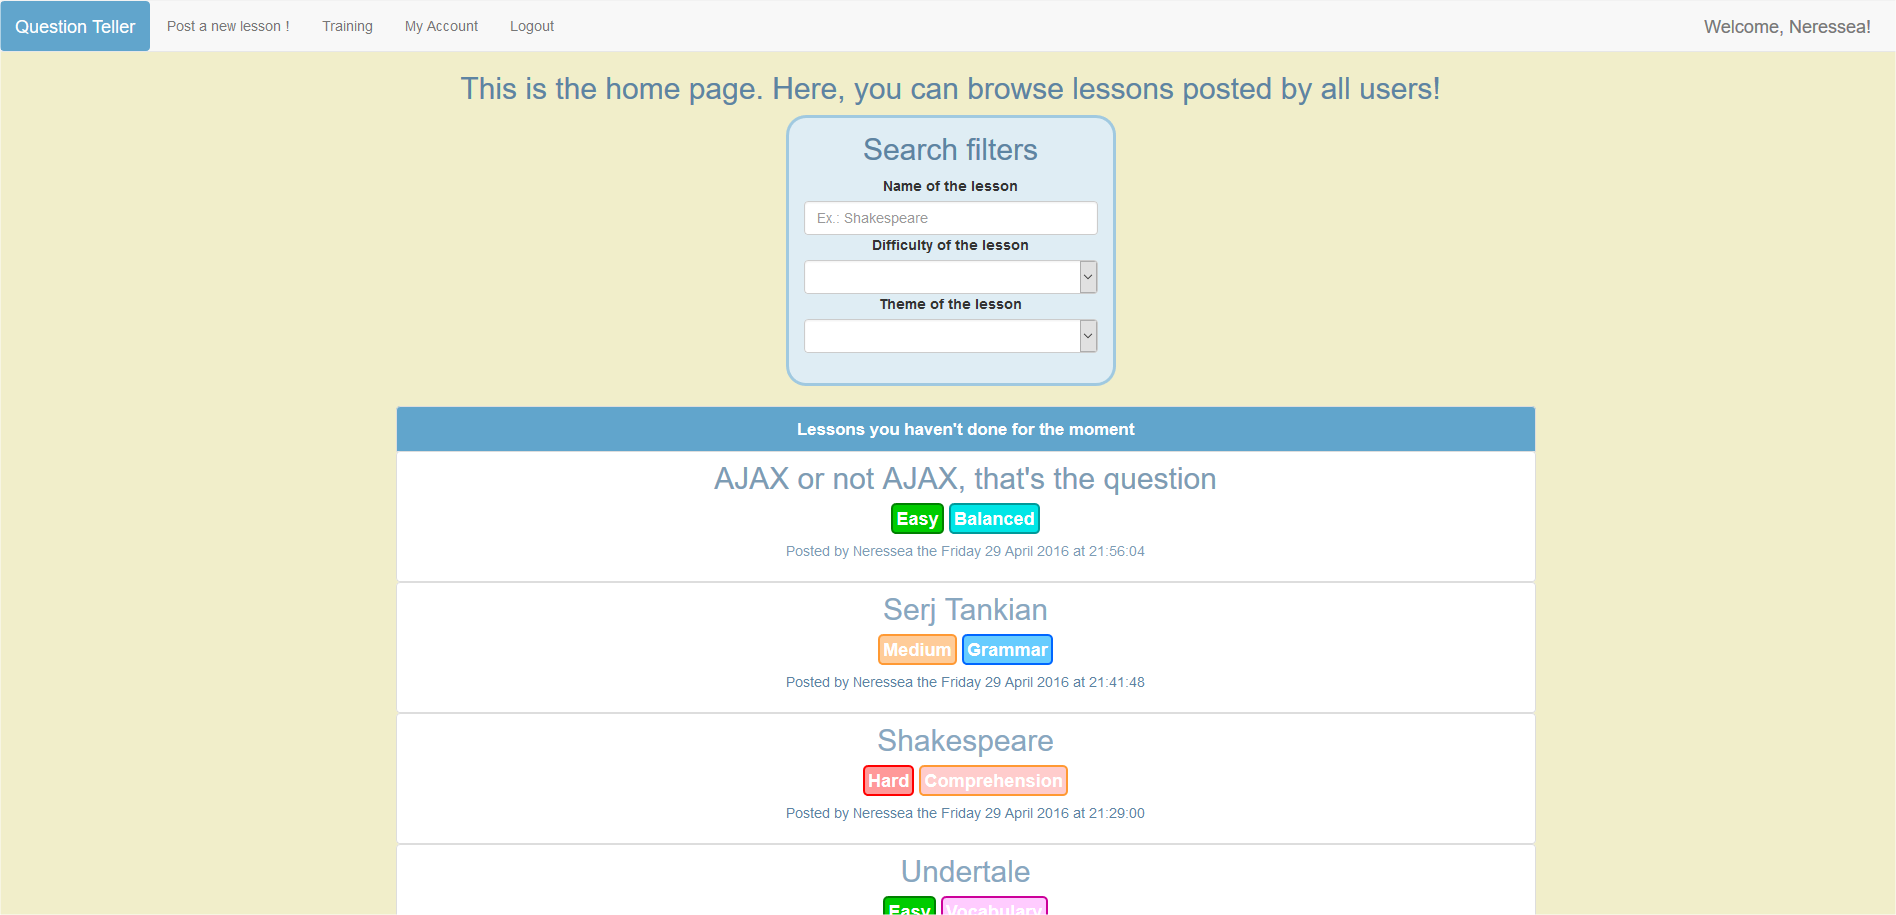
\includegraphics[width=0.5\textwidth]{./images/snapshot1.png}
    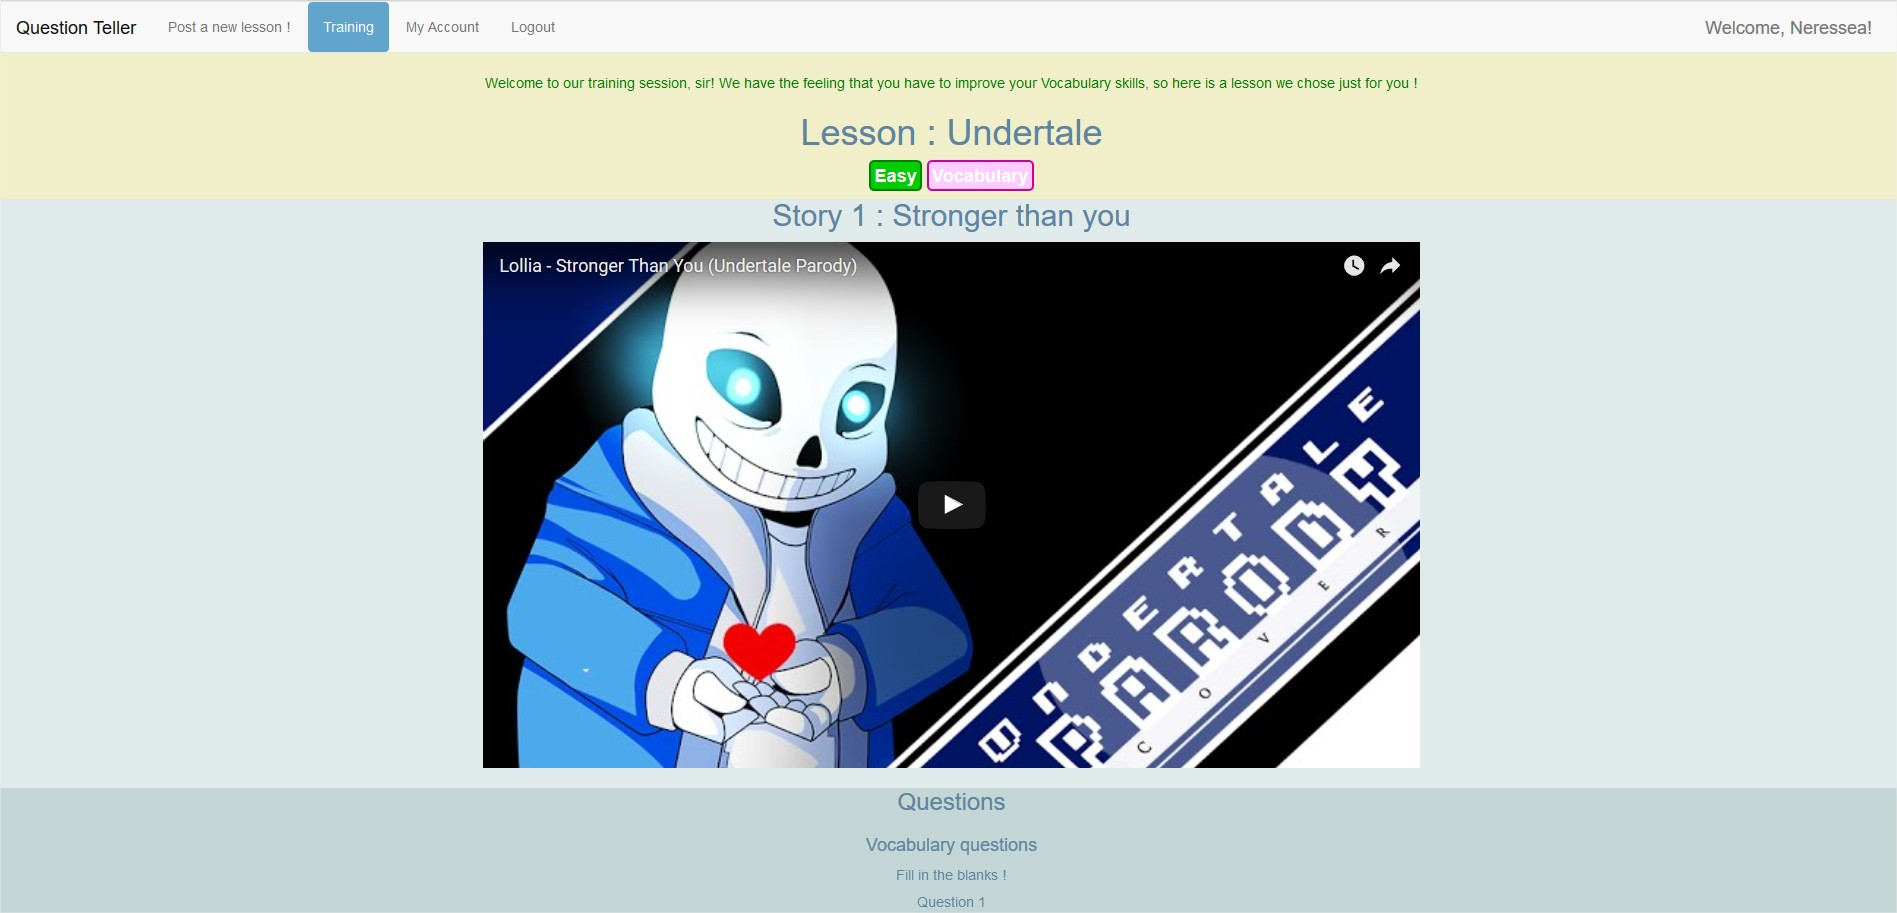
\includegraphics[width=0.5\textwidth]{./images/snapshot2.jpg}
    \caption{Snapshots of the website}
\end{figure}

\subsection{Specifications}

\paragraph{}
Thus, our objectives were to allow users to try lessons to improve themselves, each lesson being composed by several stories and questions related to it. But we didn't want to create a huge and static database of stories from the beginning. We thought it would be more entertaining if all users could create their own stories and send it to other users. But that's not all. The main feature of our application is certainly the "Training program" proposed by the server, in which the website trains the user by sending him adapted lessons.
To perform the best user experience, we also wanted the website to be responsive, so the user can either use it on a computer or a tablet. 


\paragraph{}
Now, we will see in details these different features and after that we will present you their technical side.

  \cleardoublepage
  \section{User Manual}

\subsection{The basics: How to create an account, to log in and to log out}


\subsection{Now the real thing: How to try a lesson}


\subsection{To go further: Train your english!}

\subsection{Now, you are the teacher: Post a new lesson, and help other students to improve themselves!}



  \cleardoublepage
  \section{La mise en œuvre technique du projet}

\subsection{L'organisation du projet}

Afin de travailler dans les meilleures conditions possibles, nous avons utilisé le gestionnaire de version \textbf{git} qui permet de gérer de manière approfondie le versionnage du projet et de travailler simultanément plus facilement. le projet se trouve sur le dépôt public \url{https://github.com/Neressea/EnglishProject}

\subsection{Les attentes atteintes}


\subsection{Les problèmes rencontrés et les solutions appliquées}

	
\subsection{Ce qui aurait pu être fait}
\paragraph{Les comptes administrateurs}
Bien que déjà implémenté dans la base de données, nous n'avons pas eu le temps de mettre en place les privilèges accordés aux administrateurs (édition et suppression de leçons, suppression de comptes utilisateurs).

\paragraph{Le choix du type de question}
Nous aurions pu proposer à l'utilisateur de choisir le type de question (texte à trous, QCM, question directe) désirée au lieu de décider ce type en fonction du thème de la question (vocabulaire, grammaire, compréhension).

\paragraph{Droits utilisateurs}
En l'état, un utilisateur ayant posté une leçon ne peut pas l'éditer ultérieurement. Nous aurions pu offrir cette possibilité.

\paragraph{Des réponses plus flexibles}
Les réponses données pour les questions de compréhension doivent pour l'instant être complètement identiques à la réponse entrée par l'enseignant. Les leçons seraient plus agréables pour l'élève si elles pouvaient admettre des réponses différentes ("Obama" à la place de Barack Obama, ou même des réponses très différentes mais toutes deux justes : "The president of the United States" au lieu de "Barack Obama").
  \cleardoublepage
  \section{Conclusion} % Pas de numérotation

\paragraph{}

So, we saw in the previous part that we didn't manage to implement all the features we wanted to do (like administrators rights, usage of the forgetting curve, and more flexible forms). However, we succeeded in doing the key features of this project and we think that it is sufficient to already provide a nice experience to the user. 

\paragraph{}
Besides of what we have done, this project allowed us to learn new technologies like jQuery and bootstrap, and to improve our skills in the other technologies we already knew like python, Jinja2, and straight JTML, CSS and javascript. We also had to put ourselves in the place of the user, and it was really a complicated exercise to think about everything. To have several opinions, we also asked our acquaintances to try it and tell us what they thought about it. 

\paragraph{}
As a conclusion, we think that this project was a great opportunity to explore new programming tools, and to create a real-size website during several months.
  \cleardoublepage  
  
  \thispagestyle{empty}
  \section*{Annex}
\addcontentsline{toc}{section}{Références}

\url{https://cloud.google.com/appengine/docs/python/refdocs/} \linebreak
\emph{We used python for the server.}

\url{http://jinja.pocoo.org/docs/dev/api/} \linebreak
\emph{We used a template manager to generate flexible HTML.}

\url{http://getbootstrap.com/css/} \linebreak
\emph{We used bootstrap to manipulate CSS.}

\url{http://www.w3schools.com/jsref/} \linebreak
\emph{We used javascript to manipulate the HTML from the client side.}

\url{http://texdoc.net/texmf-dist/doc/latex/latex2e-help-texinfo/latex2e.pdf} \linebreak
\emph{And finally, we used \LaTeX to write this report!} 

\end{document}

